% !TeX program = xelatex
% !BIB program = biber
\documentclass[comsoc, conference, times]{IEEEtran}

%\usepackage[subtle,bibnotes,charwidths,mathdisplays,indent,lists,tracking=normal]{savetrees}

\usepackage{amsmath}
\let\openbox\relax
\usepackage{amsthm}
\newcommand\bmmax{2}
\usepackage[cmintegrals]{newtxmath}
\usepackage{bm}

\usepackage[ruled,vlined]{algorithm2e}

% Get Booktab style ruling in algorithm blocks.
% Values shamelessly taken from egreg's answer in 
% https://tex.stackexchange.com/a/345745/82917
\makeatletter
\renewcommand*{\@algocf@pre@ruled}{\hrule height\heavyrulewidth depth0pt \kern\belowrulesep}
\renewcommand*{\algocf@caption@ruled}{\box\algocf@capbox\kern\aboverulesep\hrule height\lightrulewidth\kern\belowrulesep}
\renewcommand*{\@algocf@post@ruled}{\kern\aboverulesep\hrule height\heavyrulewidth\relax}
\makeatother

\makeatletter\let\expandableinput\@@input\makeatother

% Imports Ahoy

%\usepackage[dvipsnames]{xcolor}
%\usepackage{graphicx}
\usepackage{tikz}
\usepackage{varwidth}
\usetikzlibrary{arrows.meta, calc, fit, positioning}

%\usepackage[title]{appendix}

\usepackage{etoolbox}
\usepackage[per-mode=symbol]{siunitx}
\robustify\bfseries
\robustify\emph
%\robustify\uline
\sisetup{detect-all, range-phrase=--, range-units=single, detect-weight=true, table-format=1.3}
\DeclareSIUnit{\packet}{p}

\usepackage[super,negative]{nth}

\usepackage[british]{babel}
\usepackage{csquotes}
\usepackage{pifont}

\usepackage{booktabs}

\usepackage{xpatch}

\usepackage{url}
\usepackage[hidelinks]{hyperref}
\usepackage[nameinlink]{cleveref}
\newcommand{\crefrangeconjunction}{--}
\crefname{table}{table}{tables}

\usepackage[%
%style=ieee,minnames=1,maxcitenames=2,maxbibnames=2,
%mincrossrefs=99,minxrefs=99,
%sortcites,
maxnames=2,maxbibnames=2,mincrossrefs=99,sortcites,style=numeric-comp%
%backend=bibtex,
%uniquelist=false
]{biblatex}

\DeclareSourcemap{
	\maps[datatype=bibtex]{
		\map[overwrite]{
			\step[fieldset=urldate, null]
		}
	}
}

\addbibresource{bibliography.bib}

\DefineBibliographyStrings{english}{%
	andothers = {\emph{et al}\adddot}
}
\DeclareFieldFormat[inproceedings]{url}{}
\DeclareFieldFormat[article]{url}{}
%\DeclareFieldFormat[inproceedings]{editor}{}
%\DeclareFieldFormat[article]{editor}{}

\AtEveryBibitem{%
	\clearname{editor}%
	\clearfield{doi}%
%	\clearfield{urldate}%
%	\clearlist{urlyear}
}


\renewcommand*{\bibfont}{\footnotesize}

% Official colours!

\definecolor{uofguniversityblue}{rgb}{0, 0.219608, 0.396078}

\definecolor{uofgheather}{rgb}{0.356863, 0.32549, 0.490196}
\definecolor{uofgaquamarine}{rgb}{0.603922, 0.72549, 0.678431}
\definecolor{uofgslate}{rgb}{0.309804, 0.34902, 0.380392}
\definecolor{uofgrose}{rgb}{0.823529, 0.470588, 0.709804}
\definecolor{uofgmocha}{rgb}{0.709804, 0.564706, 0.47451}

\definecolor{uofglawn}{rgb}{0.517647, 0.741176, 0}
\definecolor{uofgcobalt}{rgb}{0, 0.615686, 0.92549}
\definecolor{uofgturquoise}{rgb}{0, 0.709804, 0.819608}
\definecolor{uofgsunshine}{rgb}{1.0, 0.862745, 0.211765}
\definecolor{uofgpumpkin}{rgb}{1.0, 0.72549, 0.282353}
\definecolor{uofgthistle}{rgb}{0.584314, 0.070588, 0.447059}
\definecolor{uofgpillarbox}{rgb}{0.701961, 0.047059, 0}
\definecolor{uofglavendar}{rgb}{0.356863, 0.301961, 0.580392}

\definecolor{uofgsandstone}{rgb}{0.321569, 0.278431, 0.231373}
\definecolor{uofgforest}{rgb}{0, 0.317647, 0.2}
\definecolor{uofgburgundy}{rgb}{0.490196, 0.133333, 0.223529}
\definecolor{uofgrust}{rgb}{0.603922, 0.227451, 0.023529}

\usepackage[T1]{fontenc}

\usepackage{FiraMono}
\setmainfont{Times New Roman}
\setmonofont[
Scale=MatchLowercase,
Contextuals={Alternate}
]{Fira Mono}

\usepackage{fontawesome5}

\usepackage[newfloat]{minted}
\usemintedstyle{tango}

\usepackage[caption=false, font=footnotesize]{subfig}

% Helpful defines
\newcommand{\ourtech}{\textsc{Galette}}
\newcommand{\afxdp}{\texttt{AF\_XDP}}
\newcommand{\af}{(\texttt{AF\_})XDP}
\newcommand{\afp}{\texttt{AF\_PACKET}}

% END Helpful defines

\newcommand{\mytitle}{\ourtech:~a~Lightweight~XDP~Dataplane on~your~Raspberry~Pi}

\usepackage{orcidlink}

\newcommand{\subparagraph}{}
\usepackage{titlesec}
\titlespacing*{\section}{0pt}{1.5ex}{0.7ex}
\titlespacing*{\subsection}{0pt}{1.5ex}{0.7ex}
\titlespacing*{\paragraph}{0pt}{1.5ex}{0.7ex}
\titlespacing*{\subsubsection}{0pt}{1.5ex}{0.7ex}

\crefformat{section}{\S{}#2#1#3}
\crefformat{subsection}{\S{}#2#1#3}
\crefformat{sections}{\S{}#2#1#3}
\crefformat{subsections}{\S{}#2#1#3}

\crefrangeformat{section}{\S{}#3#1#4--#5#2#6}
\crefrangeformat{subsection}{\S{}#3#1#4--#5#2#6}

\newcommand{\fakepara}[1]{\noindent\textbf{#1:}}

\hypersetup{
	colorlinks,
	citecolor=black,
	filecolor=black,
	linkcolor=black,
	urlcolor=black,
	pdftitle={\mytitle{}},
	pdfauthor={Kyle A. Simpson, Chris Williamson, Dimitrios P. Pezaros, Douglas J. Paul}
%	pdfauthor={Anonymous Authors}
}
\newcommand*{\email}[1]{\href{mailto:#1}{\nolinkurl{#1}}}

%\usepackage[T1]{fontenc}

\title{\mytitle}
\author{Kyle~A.~Simpson$^\dagger$$^\ddagger$~{\orcidlink{0000-0001-8068-9909}~\scriptsize[0000-0001-8068-9909]}, Chris~Williamson$^\dagger$~{\orcidlink{0000-0003-1108-9402}~\scriptsize[0000-0003-1108-9402]},\\Douglas~J.~Paul$^\dagger$~{\orcidlink{0000-0001-7402-8530}~\scriptsize[0000-0001-7402-8530]}, Dimitrios~P.~Pezaros$^\dagger$~{\orcidlink{0000-0003-0939-378X}~\scriptsize[0000-0003-0939-378X]}\\$^\dagger$\emph{University of Glasgow}, Glasgow, Scotland. $^\ddagger$\emph{Arista Networks}, Santa Clara, CA.\\\texttt{\email{kylesimpson1@acm.org}}}
%\author{Anonymous Authors\\\texttt{\email{name@domain.tld}}}

\usepackage{blindtext}

% fig spacing rules
\setlength{\abovecaptionskip}{0pt}
\setlength{\belowcaptionskip}{0pt}

\setlength{\textfloatsep}{3.0pt plus 0.0pt minus 3.0pt}
\setlength{\floatsep}{3.0pt plus 0.0pt minus 2.0pt}

\setlength{\dbltextfloatsep}{3.0pt plus 0.0pt minus 3.0pt}
\setlength{\dblfloatsep}{3.0pt plus 0.0pt minus 2.0pt}

\begin{document}
\maketitle
\begin{abstract}
%?? EMPH this feeling -- Yet we must still take advantage of advances in modern network stacks to minimise power use and reduce latency---meaning quicker response to network events, particularly in security-focussed SFCs.
	
IoT and sensor networks are now a critical part of public infrastructure.
At the same time, they remain infamous for becoming insecure as new exploits arise.
Software dataplanes give us the power to retrofit security functions, and are well-researched in datacentres.
Yet the server-grade hardware such frameworks are optimised for is a poor fit for vulnerable low-power, low-space IoT gateways.
%These environments rarely send at high data rates, and require little computational power to analyse. ?? Change focus to 'we need to reduce latency and use modern features?' still include benefits of SBCs
\emph{Single-board computers} (SBCs) are a cheaper and better fit on all these metrics, yet no \emph{service function chaining} (SFC) approaches are tailored to these devices.
%To enable this co-design
In addition, modern OS features like XDP give us the capability to minimise power use and provide the lowest latency processing these devices can offer---meaning quicker response to network events, suited to the needs of the network edge.

%While they demand little 
%or take advantage of modern OS features to offer the lowest latency processing these devices can offer.
%?? minimise power use and reduce latency---meaning quicker response to network events
%?? in a device-portable way

We present \ourtech, a device-portable SFC framework designed for the inexpensive defence of IoT networks by SBCs.
\ourtech{} builds on Linux's XDP framework to provide a CPU-efficient, low latency dataplane.
Due to SBC hardware designs, we divide traffic between an XDP fast path and userland, which lets us schedule expensive packet analysis without harming normal traffic.
Our API makes it easy to write network functions (NFs) which compile to both eBPF and native code, while being portable across heterogeneous SBCs.
Testbed evaluations show how this is more efficient, faster, and uses less power than \afp{} on Raspberry Pi.
\end{abstract}

\section{Introduction}\label{sec:introduction}
%?? Lead with the problem: need for installation of security fns etc.
IoT and sensor networks---particularly legacy installations---are infamous for their (perceived) lack of security.
Earlier devices have often been built without incorporating `security by design', leading to widespread compromise via malware like \emph{Mirai}~\parencite{DBLP:conf/uss/AntonakakisABBB17}.
Although such high-publicity mishaps have caused a sea change in how security is treated by vendors and legislation~\parencite{psti-bill}, long-term rollout of security updates can be hard to guarantee as new exploits and attacks become public.
%vendor livelihood and updates not guaranteed (plus security patches), 
Yet when the sensor networks built on such abandoned components underpin critical infrastructure,
this leaves administrators in the difficult position of having to pursue fleetwide device replacements.
This can be prohibitively expensive---particularly if these vulnerable networks are physically remote.
%This does not, however, make sensor networks built on such abandoned components any less critical; and wholesale replacement
Ideally, we desire an inexpensive and dynamically reconfigurable way to retrofit security functions into such networks with a single up-front cost as the threat landscape evolves.
%?? Want a cheap, effective way to retrofit security, reconfig as exploits and new attacks arise
%?? So, software dataplanes.

Software dataplanes are a powerful, long-standing tool for flexible network traffic processing, and offer the necessary flexibility to defend such networks.
Since \emph{Click}'s~\parencite{DBLP:conf/sosp/MorrisKJK99} debut decades ago, \emph{Service Function Chaining} (SFC) has been key in realising composable packet processing for measurement and security.
%?? for user functions and security?
The community seeks always to improve its design and performance: via accelerated network stacks like \emph{DPDK}~\parencite{DBLP:conf/ancs/BarbetteSM15}, safer language tooling~\parencite{DBLP:conf/osdi/PandaHJWRS16}, or novel hardware features like \emph{Trusted Execution Environments} (TEEs) to improve \emph{security}~\parencite{DBLP:conf/nsdi/PoddarLPR18} in untrusted, multitenant infrastructure.
%\emph{AuditBox} adds \emph{verified routing protocols} (VRPs) to this~\parencite{DBLP:conf/nsdi/LiuSKPSS21}.
As a result, we can now attest that packets are processed by the right functions without interference at high traffic rates---provided we have high-performance, well-supported hardware.

\begin{figure}
	\centering
	\resizebox{0.9\linewidth}{!}{\tikzset{
	crate/.style n args={2}{%
		append after command={\pgfextra{\let\mainnode=\tikzlastnode}
			node[above] (cc) at (\mainnode.north) {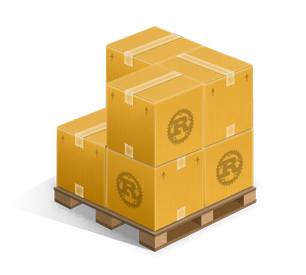
\includegraphics[keepaspectratio,width=1cm]{images/cargo}}%
			node at (cc.south) {#1}%
			node at (cc.west) {#2}%
		},
	}
}

\tikzset{
	file/.style n args={1}{%
		append after command={\pgfextra{\let\mainnode=\tikzlastnode}
			node[above] (cc) at (\mainnode.north) {\Huge\faFile*[regular]}%
			node[fill=white] at ($(cc.south) - (0,0.1)$) {\texttt{#1}}%
		},
	}
}

\tikzset{
	compile-both/.style n args={1}{%
		append after command={\pgfextra{\let\mainnode=\tikzlastnode}
			node[circle, draw, above left, fill=white] (cc) at (\mainnode) {\faMicrochip{}}%
			node[circle, draw, fill=white, inner sep=0pt,
			text width=7mm,align=center] at (\mainnode) {
\includegraphics[keepaspectratio,width=0.45cm]{images/ebpf}}%
			node[left] at (cc.west) {#1}%
		},
	}
}

\tikzset{
	compile/.style n args={1}{%
		append after command={\pgfextra{\let\mainnode=\tikzlastnode}
			node[circle, draw, above left, fill=white] (cc) at (\mainnode) {\faMicrochip{}}%
			node[left] at (cc.west) {#1}%
		},
	}
}

\tikzset{
	graphnode/.style={%
		fill=white,%
		circle,%
		draw,%
		text width=2mm,%
		align=center,%
		text=black%
	}
}

\tikzset{
	old inner xsep/.estore in=\oldinnerxsep,
	old inner ysep/.estore in=\oldinnerysep,
	double circle/.style 2 args={
		circle,
		old inner xsep=\pgfkeysvalueof{/pgf/inner xsep},
		old inner ysep=\pgfkeysvalueof{/pgf/inner ysep},
		/pgf/inner xsep=\oldinnerxsep+#1,
		/pgf/inner ysep=\oldinnerysep+#1,
		alias=sourcenode,
		append after command={
			let     \p1 = (sourcenode.center),
			\p2 = (sourcenode.east),
			\n1 = {\x2-\x1-#1-0.5*\pgflinewidth}
			in
			node [inner sep=0pt, draw, circle, minimum width=2*\n1,at=(\p1),#2] {}
		}
	},
	double circle/.default={2pt}{blue}
}

\tikzset{
	graphnode-terminal/.style n args={1}{%
		fill={#1},%
		double circle={-2pt}{#1},%
		circle,%
		draw,%
%		text width=2mm,%
		align=center,%
		text=white%
	},
	graphnode-terminal/.default={black}
}

\tikzset{
	nicebox/.style={draw,rounded corners,color=uofgsandstone,fill=uofgsandstone!10,dashed},
	gpath/.style={color=uofgheather,thick},
	usepath/.style={color=uofgmocha,thick},
	daemonbox/.style={draw, rounded corners, fill=white,align=center,},
	authbox/.style={draw, rounded corners, fill=uofgpumpkin!30, align=center,},
	client-authbox/.style={authbox,minimum width=1.8cm,rotate=90},
	authflow/.style={color=uofgthistle,thick},
	normflow/.style={color=uofgpillarbox,thick,dash dot},
}

\tikzset{
	map-cyl/.style n args={1}{%
		cylinder, shape border rotate=90, draw,align=center,aspect=0.1,font={\small},%
		cylinder uses custom fill, cylinder end fill=#1!50, cylinder body fill = #1!10
	},
	map-cyl/.default={uofgsandstone}
}

\begin{tikzpicture}
	\draw[nicebox] (0.45,-1.45) rectangle ++(3.5,2.9);
	\draw[nicebox] (-3.85,-1.4) rectangle ++(3.2,2.75);
	\node (compiler-infra) {
		\begin{tikzpicture}
			\node[crate={ACL} {a)}] (acl-crate) {};
			\node[crate={Rate Check} {b)}] at (1.5,0) (rate-crate) {};
%			\node[crate={\faLock{} DPI} {c)}] at (0, -1.5) (dpi-crate) {};
			\node[crate={DPI} {c)}] at (0, -1.5) (dpi-crate) {};
			\node[crate={Stats} {d)}] at (1.5,-1.5) (stats-crate) {};
			
			\node[draw, rounded corners, rotate=90] at (2.9,-0.25) (compiler) {\texttt{rustc} \& RedBPF};
			
			\draw[->,normflow] ($(compiler.north west) - (0.3,-0.3)$) -- ($(compiler.north west) - (0,-0.3)$);
			\draw[->,normflow] ($(compiler.north east) - (0.3,0.3)$) -- ($(compiler.north east) - (0,0.3)$);
			\draw[->,normflow] ($(compiler.south west) - (0,-0.3)$) -- ($(compiler.south west) + (0.3,0.3)$);
			\draw[->,normflow] ($(compiler.south east) - (0,0.3)$) -- ($(compiler.south east) + (0.3,-0.3)$);
			
			\node[compile-both={a)}] (acl-comp) at ($(acl-crate) + (4.75,0.4)$) {};
			\node[compile-both={b)}] (rate-comp) at ($(acl-comp) + (1.75,0)$) {};
			\node[compile={c)}] (dpi-comp) at ($(acl-comp) + (0,-1.5)$) {};
			\node[compile-both={d)}] (stats-comp) at ($(dpi-comp) + (1.75,0)$) {};
		\end{tikzpicture}
	};

	\node (chain) at ($(compiler-infra) + (-0.68, -2.7)$) {
		\begin{tikzpicture}
			\node[nicebox] (chainbox) {
				\begin{tikzpicture}
					\node[graphnode-terminal=uofgheather] (rx) {\textsc{Rx}};
					\node[graphnode] (a-node) at ($(rx) + (0,-1)$) {a};
					\node[graphnode] (b-node) at ($(a-node) + (1,0)$) {b};
					\node[graphnode] (c-node) at ($(b-node) + (1,0)$) {c};
					\node[graphnode] (d-node) at ($(b-node) + (0.5,1)$) {d};
					
					\node[graphnode-terminal=uofgpillarbox] (drop) at ($(b-node) + (2,0)$) {\tiny\textsc{Drop}};
					\node[graphnode-terminal=uofgcobalt] (tx) at ($(d-node) + (1,0)$) {\textsc{Tx}};
					
					\draw[->, gpath] (rx) -- (a-node);
					
					\draw[->, gpath] (a-node) -- (b-node);
					\draw[->, gpath] (a-node) to[out=-30, in=210] (drop);
					
					\draw[->, gpath] (b-node) -- (c-node);
					\draw[->, gpath] (b-node) -- (d-node);
					
					\draw[->, gpath] (c-node) -- (d-node);
					\draw[->, gpath] (c-node) -- (drop);
					
					\draw[->, gpath] (d-node) -- (tx);
				\end{tikzpicture}
			};
		
		\node[file={chain.toml}] (toml) at (3.5,-0.5) {};
		
		\draw[dotted, color=uofgsandstone] (chainbox.north east) -- ($(toml.west) + (-0.2,1.1)$);
		\draw[dotted, color=uofgsandstone] (chainbox.south east) -- ($(toml.west) + (-0.2,0.2)$);
		\end{tikzpicture}
	};
	
	% ------------------
	
%	\node (xdp-chain) at ($(daemon-client) + (4, -1.4)$) {
	\node (xdp-chain) at (0, -8) {\resizebox{7cm}{!}{
		\begin{tikzpicture}
			\draw[draw=black, fill=white, rounded corners] (0.3,0.3) rectangle ++(3,0.8);
			\draw[draw=black, fill=white, rounded corners] (0.15,0.15) rectangle ++(3,0.8);
			\draw[draw=black, fill=white, rounded corners] (0,0) rectangle ++(3,0.8);
			
			\node[graphnode] (c-node') at (0.5,0.4) {c};
			\node[graphnode] (d-node') at ($(c-node') + (1,0)$) {d};
			\node[graphnode-terminal=uofgpillarbox] (drop') at ($(d-node') + (1,0)$) {D};
			
			\node[graphnode] (a-node) at (0.15,-2) {a};
			\node[graphnode] (b-node) at ($(a-node) + (1,0)$) {b};
			\node[graphnode] (d-node) at ($(b-node) + (1,0)$) {d};
			
			\node[graphnode-terminal=uofgheather] (rx) at (0,-3.5) {\textsc{Rx}};
			\node[graphnode-terminal=uofgpillarbox] (drop) at ($(rx) + (1.5,0)$) {D};
			\node[graphnode-terminal=uofgcobalt] (tx) at ($(rx) + (3,0)$) {\textsc{Tx}};
			
			\node (hwt) at ($(tx) + (1,0)$) {\textsc{Hw}};
			\node[align=center] (xdpt) at ($(d-node) + (2.15,0)$) {\textsc{XDP Fast}\\\textsc{Path} 
\includegraphics[keepaspectratio,width=1em]{images/ebpf}};
			\node[align=center] (usrt) at ($(drop') + (1.8,0)$) {\textsc{User} \faMicrochip \\(\textsc{AArch64})};
			
			\draw[dashed, color=uofgsandstone] (-0.5,-1) -- (4.25,-1);
			\draw[dashed, color=uofgsandstone] (-0.5,-2.75) -- (4.25,-2.75);
			
%			\draw[dashed, color=uofgsandstone] (-0.5,-2.75) -- (-0.5,1);
%			\draw[dashed, color=uofgsandstone] (-2.25,-2.75) -- (-2.25,-3.9);
			
			\node[draw,fill=uofgsandstone!10,rounded corners,align=center] (maps) at (1.5,-1) {BPF Maps\\(State)};
			
			\draw[->, gpath] (rx) -- (a-node);
			
			\draw[->, gpath] (a-node) -- (b-node);
			\draw[->, gpath] (a-node) -- (drop);
			
			\draw[->, gpath, dashed] (b-node) to[in=-120, out=150] (c-node');
			\draw[->, gpath] (b-node) -- (d-node);
			
			\draw[->, gpath] (c-node') -- (d-node');
			\draw[->, gpath] (c-node') to[in=150, out=30] (drop');
			
			\draw[->, gpath] (d-node) -- (tx);
			\draw[->, gpath, dashed] (d-node') to[out=-30, in=90] (tx);
			
			\node[gpath, font={\small}] at ($(b-node) + (-1.55,0.5)$) {\texttt{AF\_XDP}};
			\node[gpath, font={\small}] at ($(drop') + (0.8,-1)$) {\texttt{AF\_XDP}};
			
			\draw[->, usepath] ($(maps.north) + (0, 0.4)$) -- ($(maps.north)$);
			\draw[->, usepath] ($(maps.north) + (-0.5, 0.2)$) -- ($(maps.north) - (0.2,0)$);
			\draw[->, usepath] ($(maps.north) + (0.5, 0.2)$) -- ($(maps.north) + (0.2,0)$);
			
			\draw[->, usepath] ($(maps.south) + (0, -0.4)$) -- ($(maps.south)$);
			\draw[->, usepath] ($(maps.south) + (-0.5, -0.2)$) -- ($(maps.south) - (0.2,0)$);
			\draw[->, usepath] ($(maps.south) + (0.5, -0.2)$) -- ($(maps.south) + (0.2,0)$);
		\end{tikzpicture}
	}
	};
	
	% --- dividing lines
	\draw[color=uofgsandstone!50, dashed, thick] (-5,-4.5) -- (5,-4.5);
	\node[align=center] (tee) at (4,-4.3) {\textsc{Remote Compile Server}};
	\node[align=center] (tee) at (4,-5.1) {\textsc{SBC Traffic}\\\textsc{Processor}};
	
	% --- NF flow
	\draw[->, normflow] ([yshift=0.0cm]compiler-infra.south east) to[out=-20,in=45] node[midway, below, xshift=0.8cm,yshift=0.0cm] {NF Binaries} (xdp-chain.north);
	\draw[->, normflow] (chain.south) to[out=-20,in=90] node[pos=0.3, below,yshift=-0.3cm,xshift=-1cm] {NF Config} ([xshift=-0.3cm]xdp-chain.north);
%	\draw[<->, normflow] (daemon-server.north) to[out=20,in=160] node[midway, above, fill=white,yshift=0.1cm] {NFs, Queries, Stats} (daemon-client.north);
\end{tikzpicture}}
	\caption{\ourtech{} splits traffic processing between an XDP fast path and userland, which makes the best possible use of SBC device resources. Individual NFs are written in Rust and remotely compiled to native and eBPF code, written with a single API that abstracts over runtime details.\label{fig:arch}}
\end{figure}

Yet the limited space and power available in IoT or edge deployments---to say nothing of their physical vulnerability---mean that we would be better served by inexpensive, low-power devices than by server-class hardware.
\emph{Single-Board Computers} (SBCs) like Raspberry Pis fall into this category, but are computationally weaker while lacking the hardware and driver support necessary for the above advances in SFC, like DPDK support and TEEs.
Additionally, such SBCs often run Linux, allowing us to run standard software and take advantage of advances in its kernel and network stack.%, principally network stack bypass frameworks like \af.

To our benefit, raw computational power is not always needed.
While SFCs at datacentre scale must handle millions of packets per second, data rates of IoT sensor networks can peak at \qtyrange{100}{1000}{\kilo\bit\per\second} according to industrial partners we've consulted with, while otherwise remaining mostly dormant.
However, time-critical functionality like cybersecurity functions or network fault analytics still require the minimal response times that local dataplane processing provides.
%?? DIMITRIS: want to make it sound like ``we don't need to meet Gb/s speeds, but there still is some time-critical functionality suited to DP/SBC processing''
%?? arbitrary DP programming in-situ?
This gives us scope to use SBC hardware as part of an in-situ `Goldilocks' solution, allowing administrators to choose a packet processing device with just the right size, cost, and power draw for a network's expected ingress/egress rates---without needing to steer traffic to an external cloud provider for scrubbing.
This keeps latency---and thus the reaction time to adverse security events---as low as possible.

%?? also running Linux

%?? Somewhere -- benefits and sandboxing of eBPF (\cref{sec:background})?

Where existing works look at SFC through the lens of datacentre networking, our research question is how best we can enable traffic processing on SBC devices by taking advantage of modern kernel features to implement the most performant, lowest latency dataplanes possible.
We present \ourtech{}---a device-portable SFC framework and runtime based on the modern XDP~\parencite{DBLP:conf/conext/Hoiland-Jorgensen18} and \afxdp{}~\parencite{lwn-af-xdp} network stack bypass.
\ourtech{} (\Cref{fig:arch}) explores the SFC feasibility of SBCs at various price-performance points (e.g., Raspberry Pis and Intel NUCs), and provides a consistent platform for all Linux-capable SBCs.
We use a two-tier strategy, splitting \emph{network functions} (NFs) between XDP and userland.% due to the limited number of receive queues on SBCs. ?? Check DIMITRIS NOTE
NFs are written in \emph{Rust}~\parencite{rust} against a simple API, and are compiled on a remote control node into both native and eBPF binaries.
However, \af{}'s true value for SBC devices is that its performance scales gracefully with driver support, which buys improvements like zero-copy and elimination of SKB allocation.
Our framework requires only a modern Linux version, and benefits from the strong sandboxing and validation of eBPF (\cref{sec:background}).
While primarily designed for retrofitting cybersecurity, our work can also be used for arbitrary NFs such as secure tunnelling of traffic~\parencite{electric-imp}, local reduction of sensor and telemetry data for external processing~\parencite{DBLP:conf/globecom/SimpsonCP20}, or compressed ML/RL models~\parencite{DBLP:conf/noms/SimpsonP22,DBLP:conf/nsdi/SiracusanoGSMAC22}.

% \emph{\`a la} ElectricImp~\parencite{electric-imp}. ?? Good although should not assume widely known -- tie into Seidr~\parencite{DBLP:conf/globecom/SimpsonCP20}, or Opal~\parencite{DBLP:conf/noms/SimpsonP22} here?
%Pure-XDP chains also portable.

%Due to various factors, 
%
%?? Rust NFs, single API
%?? Requires only as recent linux kernel, scales with...
%
%?? Quickly explain new stack bypasses in modern linux.
%\Cref{fig:arch}
%
%%Raspberry Pis and many NUCs 
%% Maximal performance out of cheap boxen.
%%?? Can we push 
%
%?? Note on state of other XDP-based works.
%?? Target datacentre networks: hardware support for multiple receive queues. SBCs don't have this, don't always have DPDK support (needs driver support), same with other packet processing frameworks?
%?? But also multicore, need to take best advantage even if the kernel won't let us.
%?? ``Existing works look at service function chaining through the lens of datacentre networking''
%
%%?? What features don't we have on small boxes, what must we design around?
%%?? No SGX, Trusted Exec Environments
%
%?? Primarily designed for security NFs, reconfigability, but can also be used for tunnelling of traffic etc. \emph{\`a la} ElectricImp~\parencite{electric-imp}.
%
%?? True value of XDP/\afxdp{}? Performance scales gracefully according to driver support, NOT all or nothing. Driver support buys improvements like zero-copy, and native XDP rather than SKB-based. So device portable, all that's needed is modern Linux. Pure-XDP chains also portable.
%
%
%
%?? Misc lines from notes:
%?? Pareto-optimal point between power use, cost, performance.


\subsection{Contributions}
This paper contributes:
\begin{itemize}
	\item an analysis of the differences between SBC and server hardware which prevent us from taking full advantage of XDP (\cref{sec:motivation}),
	\item control- and data-plane designs built on \af{} to allow efficient SFC installation, reconfiguration, and scheduling on SBCs in spite of these differences (\cref{sec:design}),
	\item a simple API and chain format for building SFCs to target both eBPF and userland environments (\crefrange{sec:design:chain}{sec:nf-api}),
	\item a quantitative evaluation of the forwarding performance and resource use of \ourtech{} against other usable software dataplanes in SBCs, as well as how our two-tier design allows effective loadbalancing and scheduling of expensive NFs (\crefrange{sec:evaluation}{sec:results}).
\end{itemize}
%Additionally, we... (expand somewhat).

\section{Background}\label{sec:background}

\fakepara{eBPF}
The \emph{extended Berkeley Packet Filter} (eBPF) is a simple RISC VM bytecode language used to execute arbitrary user-written code in Linux kernel contexts at runtime~\parencite{ebpf-history}.
eBPF programs can be attached to various \emph{hooks} or \emph{tracepoints} in the kernel for precise instrumentation or additional control over, e.g., network stack behaviour.
Each valid kernel hook exposes a different set of BPF helpers---a limited set of privileged operations allowed by the kernel in a given function, such as buffer manipulation or adjusting the header pointer for a packet SKB.
Programs are restricted similarly to constrained embedded targets: dynamic memory allocation is impossible, and there is no support for floating point arithmetic.
Programs may hold state between invocations or share it with userland code via \emph{BPF Maps}, which abstract over arrays, hash maps, and more specialised structures like longest-prefix match tries.
%?? State via BPF Maps.

The Linux kernel does some heavy lifting to ensure this functionality is safe and performant.
The main mechanism for doing so is its \emph{eBPF Verifier}, which ensures that all pointer and map accesses are length-checked and that the program is guaranteed to terminate in a bounded time.
Programs themselves are each limited to \num{4096} instructions, \qty{512}{\byte} of stack space, and may be linked via tail-calls up to a maximum \num{32} programs.
Additionally, all used BPF helpers must be permitted by the call site, and only pointers supplied by the kernel (or maps) have the type and length information needed to be dereferenced.
Kernel versions 5.3 onwards allow for the use of trivially bounded loops without unrolling. %~\parencite{bpf-loops}.
Following verification, BPF programs are JIT-compiled for the host architecture by translating BPF instructions to their native machine code equivalents---program code is then further hardened by write protecting memory and constant blinding to prevent the insertion of exploitable native code gadgets~\parencite{jit-spraying-bpf}.

\fakepara{XDP}
The \emph{eXpress Data Path} (XDP) is a network-stack bypass mechanism for Linux, allowing eBPF programs to handle network packets at the earliest possible stage in the kernel~\parencite{DBLP:conf/conext/Hoiland-Jorgensen18}.
XDP hooks may modify packet contents and adjust header lengths (enabling en/decapsulation), and may quickly redirect packets to be transmitted on their arrival port or any other NIC.
Packets may also be redirected to other registered XDP hooks via eBPF tailcalls, or to the standard network stack.
The stack bypass is completed by \afxdp{}~\parencite{lwn-af-xdp}, which allows packets to be passed from XDP hooks to userland, allowing packets which need more complex processing to entirely skip the Linux network stack.
This follows a netmap-like design~\parencite{DBLP:conf/usenix/Rizzo12}, passing UMEM frame descriptors between contexts using a set of ring buffers.
%These technologies have been key in the recent redesign of \emph{Open vSwitch}~\parencite{DBLP:conf/sigcomm/TuWAP21} and high-performance load balancers like \emph{Katran}~\parencite{katran}.
To take advantage of multicore systems and scale to high packet rates, XDP runs one eBPF context in parallel for each hardware receive queue exposed by a NIC.

XDP is particularly valuable compared to other stack or kernel bypass approaches like \emph{DPDK}~\parencite{dpdk} because it does not require dedicated driver support.
All NICs are supported by default by placing the eBPF program after SKB allocation; performance benefits scale gracefully with driver support, enabling the hook to run \emph{before} SKB creation or in a zero-copy mode.
%?? SKB mode, all the way to physical offload.
Capable hardware like SmartNICs~\parencite{netronome-smartnic} or \emph{hXDP}~\parencite{DBLP:conf/osdi/BrunellaBBPSBCP20} may even offload eBPF code to the NIC for true kernel bypass.

%?? Also soon to be supported on Windows~\parencite{xdp-windows}.

%?? Fit \emph{netmap}~\parencite{DBLP:conf/usenix/Rizzo12} into above? I.e., unlike DPDK and netmap...

\section{Motivation}\label{sec:motivation}
While \af{} SFC frameworks are well-studied (\cref{sec:related}), SBCs---particularly those in edge or IoT networks---are differentiated from datacentre or cloud environments in key ways that existing frameworks do not account for:
\begin{itemize}
	\item \emph{Raw compute performance and resources.}
	SBCs such as Raspberry Pis have slower CPU clocks, fewer cores, and less RAM then server-grade hardware, making it harder to run more costly NFs within packet deadlines.
	However, this further amplifies the impact of host networking stack overheads on packet processing latency and throughput.
	This ties into two useful counterpoints raised in \cref{sec:introduction}: IoT and sensor networks exhibit low (sub-\unit{\mega\bit\per\second}) data rates, so low-power processing nodes are an ideal fit; equally, the lower up-front cost of these platforms makes them more attractive for installation in vulnerable and remote environments.
	Yet we must still take advantage of advances in modern network stacks to minimise power use and reduce latency---meaning quicker response to network events, particularly in security-focussed SFCs.
	
	\item \emph{Rx/Tx queues and use of NIC virtual functions.}
	XDP's degree of parallelism scales according to the number of Rx queues exposed by a NIC.
	Datacentre NICs targeting 10GbE and above allow Rx queues and virtual functions to be created on demand, thus XDP-based frameworks can easily scale to have as many pipelines as are required to meet bandwidth needs.
	%	?? Eh, something about how frameworks scale up using these to hit BW reqs.
	On the contrary, we find that GbE and below NICs common to SBCs---including those with DPDK support, such as the Intel I219-V---expose only a single Rx/Tx queue.
	Though many SBCs are multicore devices, this mismatch prevents the XDP datapath from scaling to fit these extra cores.
	As a result, SFCs on this single pipeline are vulnerable to tail latency spikes and throughput losses caused by \emph{more expensive NFs which may only be needed by a subset of traffic}.
	%	?? Pipeline stall impact, control over load balancing, ... 
	%	?? tail latencies from stalls.
\end{itemize}

%?? Need agility to update, reconfigure chains. Smaller programs due to eBPF program limits.
A concrete use case is in how an SBC-based SFC framework could be used to secure legacy IoT or sensor networks at minimal cost, as in \cref{sec:introduction}.
%Older IoT devices are infamous for placing security as an afterthought, and questionable long-term support for (often Linux-based) devices can lead to edge devices \emph{becoming} insecure as new exploits are discovered---original manufacturers may cease trading or prefer that administrators repurchase the newest model.
%Recall that the (often Linux-based) devices can \emph{become} insecure as new exploits are discovered if security updates cease.
Assuming exploit-based attacks rather than volumetric DDoS traffic (which would have to to effectively be dealt with upstream), the majority of network packets traversing an IoT gateway are likely to be normal, and should not require complex processing like \emph{deep packet inspection} (DPI)---which would block an SBC's sole XDP thread.
Most importantly, we need a framework with the agility to install, update, and reconfigure chains of NFs to defend against attacks as they evolve.
%?? Attacks, desired NFs \& their interconnections change.
%Moreover, ...

%?? Tie in the security use-case here?
%?? Explicitly mention cheaper first-stage analyses, linked into e.g. ML model only as needed.
%?? Semantic and protocol attacks rather than DDoS -- which



%?? Requirements -- what differentiates SBC machines from datacentre or cloud-centric frameworks? Rx/Tx queues and use of VFs. Also clock rate, power, memory, space, volatility...

\section{Design}\label{sec:design}
%?? Headline of design -- high-level summary and why.

We present here our design and implementation for \ourtech{}, which takes advantage of advances in Linux host networking---XDP---to provide a portable, device independent framework for deploying SFCs onto modest-spec heterogeneous devices irrespective of machine architecture.

We use a hybrid XDP and userland solution to bring low-latency SFCs to inexpensive SBC hardware, enabling the retrofitting and modification or defence of IoT \& sensor networks (\cref{fig:arch}).
Chains are composed of individual crates written in Rust---each compiled to \emph{both eBPF and native machine code} by a remote control plane machine---against a simple API which unifies packet accesses in both environments.
This enables easy dual compilation into both eBPF and native machine code while guaranteeing memory safety, but crucially allows one chain to compile to SBCs with different CPU architectures.
Userland-only (\emph{non \ourtech-native}) NFs may link to external C libraries.
As modern SBCs are multicore but their NICs typically support only a single XDP thread, we push expensive or complex NFs (possibly required by only a subset of traffic) out of the main datapath to exploit extra cores for load balancing while eliminating packet stalls and minimising extra latency.

\subsection{Chain format}\label{sec:design:chain}
SFCs are defined by administrators via a user-friendly TOML format, which affords control over BPF map definitions as well as where individual NFs are run.
\Cref{listing:chain-sec} shows a practical example of a security-focussed chain: packets are processed by an ACL backed by an LPM trie map, while suspicious packets are also checked by a cheaper statistical classifier which may trigger an expensive DPI operation in userland.
Any map may be shared between NFs by pointing to a \mintinline{toml}|[maps.<x>]| block.

\begin{listing}
	\centering
	\inputminted[fontsize=\footnotesize]{toml}{listings/security.toml}
	\caption{A security-focussed function chain. Cheaper classification is kept in the XDP datapath, while expensive analyses are pushed into userland.\label{listing:chain-sec}}
\end{listing}

Every chain starts from \mintinline{rust}|"rx"|, and routes from there to its NFs and the special destinations \mintinline{rust}|"tx"|, \mintinline{rust}|"pass"|, \mintinline{rust}|"abort"|, and \mintinline{rust}|"drop"|.
%\footnote{Our current dataplane prototype does not support transmitting data from one interface to another (i.e., \mintinline{toml}|to = ["tx(eno2)"]|), although XDP itself easily allows this. We consider this a useful future extension.}
These correspond to most of the standard XDP actions---\mintinline{c}|XDP_PASS| forwards a packet to the standard host networking stack, and is useful if control plane traffic must be sent in-band (i.e., a bump-in-the-wire installation at a site with poor cellular service).
The number of valid \mintinline{toml}|to| destinations is determined and checked during code generation (\cref{sec:compilation}).

\Cref{listing:chain-sec} also demonstrates two ways that users can manage the placement of NFs---they may explicitly run any NF in userland with the \mintinline{rust}|"!dest"| syntax, or set \mintinline{toml}|disable_xdp = true| to do this implicitly and skip eBPF compilation (\cref{sec:compilation}).
Control over these mechanisms is explicit to allow users to define pure XDP chains and avoid cross-compilation, or to effortlessly load-balance a single chain between userland and XDP.
The exception is that calls are forcibly moved to userland if the chain length exceeds \numlist{32} NFs.

%?? users specify XDP friendliness
%?? can point to other folder.

\subsection{Shared NF API}\label{sec:nf-api}
Compiling to eBPF requires that we mark an NF's crate as \mintinline{rust}|#![no_std]|, yet there are standard functions that NF authors desire use of like random number generation, timestamping, map declaration/access, and packet headroom adjustments.
Also, though both NF environments provide packet access via a byte buffer, the eBPF verifier requires that packet accesses are length checked in a particular way to pass static verification (i.e., such that Rust's pointer-length slices are inadequate).
To this end, we provide a small standard library and a family of traits which enable programmers to write \ourtech-native NFs.

\begin{listing}
	\centering
	\inputminted[fontsize=\footnotesize]{rust}{listings/macswap.rs}
	\caption{A counting macswap function in \ourtech. \ourtech-native NFs are written in Rust with a simple API shared between eBPF and native targets.\label{listing:macswap}}
\end{listing}

%This says nothing of other ``standard-lib like functionality''
\Cref{listing:macswap} shows how a simple MAC swapping NF is implemented in \ourtech.
The \mintinline{rust}|Packet| trait abstracts over different packet access semantics in userland and XDP, implemented for UMEM frames and XDP contexts, respectively.
Handling of maps requires a custom procedural macro, \mintinline{rust}|#[maps]|, which converts \mintinline{rust}|(K,V)| pairs into generic \mintinline{rust}|Map<K,V>|s and exposes these types such that they can be programmatically manipulated when building concrete NF skeletons for each target.

%?? User-only NFs can make use of std functionality -- maybe also can use specialised or non-POD data storage.
Userland-only NFs do not require the \mintinline{rust}|#![no_std]| tag, and are thus free to call standard library functions, as well as link to and call precompiled libraries and native code.
This frees users from having to reimplement complex well-tested NFs, but also allows administrators to limit and reason about the unsafety of (possibly proprietary) C codebases.
These currently use eBPF maps, and so key/value types must be plain-old-data structs.
In future these NFs could instead be given direct access to efficient userland shared data structures. % like \emph{DashMap}~\parencite{dashmap}.

%?? Source code in new language not always needed. can use existing pre-compiled libraries can be linked in to userland dylibs -- can scope and limit C code, proprietary black boxes and their (un)safety in this way. (``reason about the impact and effects of <x> this way?'')

\subsection{Compilation}\label{sec:compilation}
SBCs lack the resources to (re-)compile NFs. %; doubly so when using the Rust compiler, which is known to be computationally demanding.
Compilation of NFs in an SFC is thus performed by an external controller machine which is trusted from the outset (\cref{sec:ctl-plane}), where eBPF binaries (``.elf'') and dylibs (``.so'') are incrementally sent over the network.
The root \texttt{lib.rs} file for each NF is parsed into an AST using the `syn' library, from which we extract:
\begin{itemize}
	\item the type name of the first \mintinline{rust}|struct| decorated with \mintinline{rust}|#[maps]| plus its number of fields, and
	\item the return type of the main \mintinline{rust}|packet()| function as well as the number of \mintinline{rust}|enum| variants it has.
\end{itemize}
We compare this against the chain definition file to ensure that there is a one-to-one correspondence between these and the expected number of maps and output branches.
From this, we then generate source code and crates which compile to an eBPF program and dylib.
Userland NFs require little additional code.
Generation of XDP NFs is slightly more involved: we insert a declaration for each map required by user code (with key and value types exposed and inserted via the NF API---\cref{sec:nf-api}), allocate maps for \afxdp{} sockets, and storage for NF chain actions and next hops via the \mintinline{rust}|PROG_ARRAY| map type.

%?? FOrgot -- this occurs OFF DEVICE, and is sent over ctl plane.

%?? Map declarations: Parse NF, read number of outputs, compare against instances in chain.toml, allocate ProgMap and ActionSet (map to XDP actions + upcall) of size next PoT. Size-1 entries for dataplane state. XskMap of size 8 for upcall sockets.
%
%?? Mention in upcalling -- no memcpy happens on the adjust headroom!!
%
%?? Correctly monomorphised with \mintinline{rust}|Map| and \mintinline{rust}|Packet| types according to callsite.

\subsection{Dataplane operation}

\begin{figure}
	\centering
	\resizebox{0.9\linewidth}{!}{\tikzset{
	nicebox/.style={draw,rounded corners,color=uofgsandstone,fill=uofgsandstone!10,dashed},
	nfbox/.style={draw,rounded corners,color=uofgsandstone,fill=uofgsandstone!5},
	nfbox2/.style={nfbox, fill=uofgsandstone!1},
	gpath/.style={color=uofgheather,thick},
	usepath/.style={color=uofgmocha,thick},
	daemonbox/.style={draw, rounded corners, fill=white,align=center,},
	authbox/.style={draw, rounded corners, fill=uofgpumpkin!30, align=center,},
	client-authbox/.style={authbox,minimum width=1.8cm,rotate=90},
	authflow/.style={color=uofgthistle,thick},
	normflow/.style={color=uofgpillarbox,thick,dash dot},
	readflow/.style={color=uofgcobalt,thick,dash dot},
}

\begin{tikzpicture}
\draw[nfbox, opacity=0.3] (-3.0,-1.5) rectangle ++(7,3.2);
\draw[nfbox2] (-2.9,-1.4) rectangle ++(7,3.2);
\draw[nfbox] (-2.8,-1.3) rectangle ++(7,3.2);
	
\node (test) {
	\begin{tikzpicture}
	\node (name) {
\includegraphics[keepaspectratio,width=1em]{images/ebpf} \textbf{NF \emph{a}}};
	
	\node[draw, rectangle, align=left] (b1) at ($(name) + (1, -0.75)$) {\mintinline{rust}|nf(ctx.body)|};
	\node[draw, rectangle, align=left] (b2) at ($(b1) + (0,-0.8)$) {Get action};
%	\node[draw, rectangle, align=left] (b3) at ($(b2) + (0,-0.55)$) {Write ID};
%	\node[draw, rectangle, align=left] (b4) at ($(b3) + (0,-0.55)$) {Redirect to \afxdp{}};

	\node[draw, rectangle, align=left] (b3) at ($(b2) + (0.75,-1)$) {Write IDs};
	\node[draw, rectangle, align=left] (b4) at ($(b3) + (2.75,0)$) {Redirect to \afxdp{}};
	
	\node (tab) at ($(b1) + (3.5, -0.25)$) {
		\resizebox{3cm}{!}{\begin{tabular}{ccc}
			\toprule
			Result $\circledast$ & Action & \texttt{PROG}\\
			\midrule
			0 & \texttt{Tx} & --- \\
			1 & \texttt{Call} & NF \emph{b} \\
			2 & \texttt{Upcall} & --- \\
			\bottomrule
		\end{tabular}}
	};

	\draw[->, authflow] (b1.south west) to[out=210,in=180] node[midway, left, xshift=0.05cm, yshift=0.3cm] {$\circledast$} (b2.west);
	\draw[->, authflow] (b2.south) to[out=250,in=160] node[midway, right, yshift=0.15cm] {\texttt{Upcall}} (b3.west);
	\draw[->, authflow] (b3.east) -- (b4.west);
	\draw[->, authflow] (b2.south) to[out=250,in=0] node[midway, right, yshift=0.15cm, xshift=-2cm] {\texttt{Tx, Drop}} ($(b2.south) + (-2.5, -1)$);
	\draw[->, authflow] (b2.south west) to[out=210,in=180] node[midway, below, align=center, xshift=-0.5cm, yshift=0.2cm] {\texttt{Call}\\\texttt{NF}} ($(name.west) + (-0.25, 0)$);
	\draw[->, authflow] (b4.south) to[out=270,in=0] node[midway, below, align=center, xshift=-1cm, yshift=0.15cm] {\texttt{Tx}} ($(b4.south) + (-1, -0.5)$);
	
	\draw[->, readflow] (tab.west) to node[midway, below, xshift=0.4cm, yshift=0.1cm] {\footnotesize\texttt{get($\circledast$)}} (b2.east);	
	\end{tikzpicture}
};

\node (xsks) at (5.5,0.25) {
	\begin{tikzpicture}
		\node[opacity=0.1] at (0.3,-0.3) {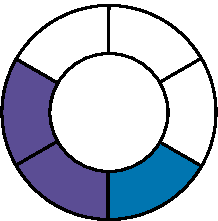
\includegraphics[keepaspectratio,width=3em]{images/ringbuf}};
		\node[opacity=0.25] at (0.2,-0.2) {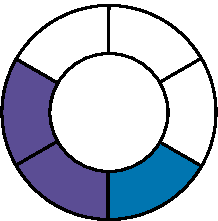
\includegraphics[keepaspectratio,width=3em]{images/ringbuf}};
		\node[opacity=0.5] at (0.1,-0.1) {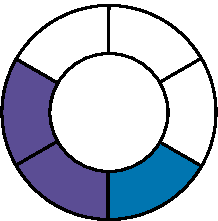
\includegraphics[keepaspectratio,width=3em]{images/ringbuf}};
		\node at (-0,0) {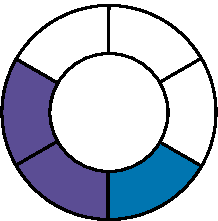
\includegraphics[keepaspectratio,width=3em]{images/ringbuf}};
	\end{tikzpicture}
};

\node[align=center] (xsk-lab) at ($(xsks) + (-0.1,-1.2)$) {\afxdp\\Sockets (XSKs)};

\node[color=uofgrust] (xdp-text) at ($(test) + (-0.9,2.3)$) {\large\texttt{\textbf{Entry:} XDP hook}};
\draw[->, authflow] (xdp-text) to[out=-45,in=45] ($(xdp-text) + (0, -1)$);

\draw[->, readflow] ($(xsks.west) + (0.1,0)$) to node[midway, below, xshift=-1.4cm, yshift=0cm] {\footnotesize\texttt{get(rand())}} ($(xsks.west) + (-0.9,-0.9)$);
\end{tikzpicture}}
	\caption{Packet processing in the XDP Fast Path (NF maps omitted).\label{fig:dplane-xdp}}
\end{figure}

\fakepara{XDP (\cref{fig:dplane-xdp})}
On arrival, the main body of the NF is executed and its output is used as an index to the map of actions defined by the chain---e.g., \texttt{XDP\_TX}/\texttt{DROP}, NF calls.
Although eBPF maps have a small runtime lookup cost, we make use of them to store action mappings to enable dynamic, fast reconfiguration without needing to recompile any NFs.

When calling another NF, we perform an XDP tail-call into a \mintinline{rust}|PROG_ARRAY| using the same index.
When upcalling to userland via \afxdp, packets arrive without explicitly including XDP state but do include user-defined metadata.
As \afxdp{} sockets rely on \emph{single-producer-single-consumer} (SPSC) rings to move frames between userland and the kernel, we create one socket per running userland thread and load balance between them using the \mintinline{c}|bpf_get_prandom_u32()| helper function.
However, as any chain allows many discrete XDP$\rightarrow$Userland transitions, we need to signal the identity of the callee NF so that packet processing can resume.
To work around this we assign a unique ID to each live NF.
When an upcall is required, we expand a packet's metadata by \qty{8}{\byte} to store this ID and the action index---inspecting the kernel source code, this resolves to a cheap pointer adjustment within the larger headroom block rather than a \texttt{memcpy}.
%XDP metadata is typically used to pass state between eBPF programs, but is used here because it is visible to recipients over \afxdp{}.

%?? As focus is dynamic, fast reconfig without recompile, then we have a big action map.

\begin{figure}
	\centering
	\resizebox{0.8\linewidth}{!}{\tikzset{
	nfbox/.style={draw,rounded corners,color=uofgsandstone,fill=uofgsandstone!5},
	membox/.style={draw,color=uofgsandstone,fill=uofgsandstone!5},
	idbox/.style={draw,color=uofgpillarbox,fill=uofgpillarbox!5},
	actbox/.style={draw,color=uofgpumpkin,fill=uofgpumpkin!5},
	authflow/.style={color=uofgthistle,thick},
	putflow/.style={color=uofgpillarbox,thick,dash dot},
	readflow/.style={color=uofgcobalt,thick,dash dot},
	zoomflow/.style={color=uofgcobalt!50,thick,dotted},
}

\begin{tikzpicture}
\node (rxq) {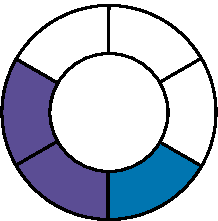
\includegraphics[keepaspectratio,width=3em]{images/ringbuf}};
\node (rxq-l) at ($(rxq) + (0,-0.75)$) {Rx};

\node (txq) at ($(rxq) + (0,-1.5)$) {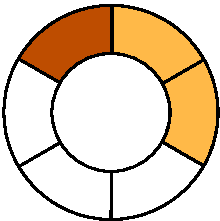
\includegraphics[keepaspectratio,width=3em]{images/ringbuf-alt}};
\node (txq-l) at ($(txq) + (0,-0.75)$) {Tx};

\node (cq) at ($(txq) + (0,-1.5)$) {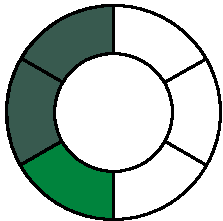
\includegraphics[keepaspectratio,width=3em]{images/ringbuf-alt2}};
\node (cq-l) at ($(cq) + (0,-0.75)$) {Completion};

\node (umem) at ($(rxq) + (3.5,0)$) {
	\begin{tikzpicture}
		\node[rotate=90] (umem-label) at (0,0) {\textsc{Umem}};
		\draw[membox, opacity=0.5] ($(umem-label) + (0.25,0.25)$) rectangle ++(4,0.25);
		\draw[membox] ($(umem-label) + (0.25,0)$) rectangle ++(4,0.25);
		\draw[membox, opacity=0.5] ($(umem-label) + (0.25,-0.25)$) rectangle ++(4,0.25);
		\draw[membox, opacity=0.5] ($(umem-label) + (0.25,-0.5)$) rectangle ++(4,0.25);
		
		\draw[actbox] ($(umem-label) + (0.25,0)$) rectangle ++(1.5,0.25);
		\draw[idbox] ($(umem-label) + (0.25,0)$) rectangle ++(0.75,0.25);
		
		\node[color=uofgpillarbox] at ($(umem-label) + (0.62,0.125)$) {\scriptsize{NF ID}};
		\node[color=uofgpumpkin!50!uofgpillarbox] at ($(umem-label) + (1.38,0.125)$) {$\circledast$};
		\node[color=uofgsandstone] at ($(umem-label) + (3,0.11)$) {\scriptsize{Packet Body}};
	\end{tikzpicture}
};

\node[draw, rectangle, align=left] (b1) at (3.5,-1) {Get packet(s)};
\node[draw, rectangle, align=left] (b2) at ($(b1) + (0,-0.8)$) {\texttt{next\_nf(ID,$\circledast$)}};
\node[draw, rectangle, align=left] (b3) at ($(b2) + (0,-0.8)$) {\texttt{nf\_dylib(pkt,$\triangle$)}};
\node[draw, rectangle, align=left] (b4) at ($(b3) + (0,-0.8)$) {Cleanup};

\node (nfs) at (7,-2.5) {
	\begin{tikzpicture}
		\draw[nfbox, opacity=0.25] (0.2,-0.2) rectangle ++(1,1);
		\draw[nfbox, opacity=0.5] (0.1,-0.1) rectangle ++(1,1);
		\draw[nfbox] (0,0) rectangle ++(1,1);
		
		\node at (0.5,0.4) {\faMicrochip};
		\node at (0.35,0.85) {\scriptsize{\textbf{NF \emph{b}}}};
	\end{tikzpicture}
};

\draw[-,zoomflow] (0.22,-0.18) -- (1.4,0.24);
\draw[-,zoomflow] (0.4,-0.24) -- (1.4,0);

\draw[->, authflow] (b1.east) to[out=-10,in=90] (b2.north east);
\draw[->, authflow] (b2.east) to[out=-10,in=10] node[midway, right] {$\triangle$} (b3.east);
\draw[->, authflow] (b3.south west) to[out=-180,in=180, parabola height=1cm] node[midway, left, sloped, yshift=0.25cm, xshift=0.75cm] {\texttt{Call:} $\triangle'$} (b3.north west);
\draw[->, authflow] (b3.south east) to[out=-30,in=10, parabola height=1cm] (b4.east);

\draw[->, authflow, opacity=0.25] (b4.west) to[out=-180,in=-180, parabola height=-5cm] (b1.west);

\draw[->, readflow] (rxq) to node[midway, below, xshift=-0.4cm] {\footnotesize\texttt{read()}} (b1.west);
\draw[->, readflow] (nfs) to node[midway, below] {\footnotesize\texttt{get($\triangle$)}} (b3.east);

\draw[->, putflow] (b4) to[out=-170, in=-30] node[midway, below] {\footnotesize\texttt{Drop}} (cq);
\draw[->, putflow] ($(b3.west) + (-0.55,0)$) to node[midway, below] {\footnotesize\texttt{Tx}} (txq);
\end{tikzpicture}}
	\caption{Packet processing in userland (single-thread, NF maps omitted).\label{fig:dplane-user}}
\end{figure}

\fakepara{Userland (\cref{fig:dplane-user})}
Packets are received on the Rx ring of each userland thread's \afxdp{} socket, and XDP metadata is read from the UMEM frame to establish the callee and target NFs.
This allows us to look up the function pointer given by the required NF's dynamic library, and packets are then processed by run-to-completion.
%?? Ring bufs between userland threads 2--$n$.
%?? Run-to-completion, dylibs til done.
%?? No way to pass packets back down, so even eBPF-compatible NFs must be duplicated at this layer.
We choose this model as there is no native mechanism to pass packets back to XDP---subsequent \ourtech-native NFs are also executed as dylibs (which can be better-compiled than the in-kernel JIT).
Some other XDP-based approaches like \emph{Polycube}~\parencite{DBLP:journals/tnsm/MianoRBBL21} choose to downcall using a TAP device after \emph{every} `slow-path' NF executes. 
We choose not to pay the extra repeated overhead needed to do so, while also keeping packet pressure off the sole XDP fast-path thread.

As SBC hardware allows us to bind only a single Rx queue for XDP, we are forced to use a single UMEM pool between all \afxdp{} sockets.
In turn, UMEM frame cleanup and recycling can only occur on a single thread.
We delegate these tasks to the first userland thread, using ring buffers between it and threads 2--$n$ to correctly handle packet drop/abort actions.

%?? DIMITRIS: diagram for above 2 paras?

%\fakepara{Rest}
%
%?? Lifecycle of a packet?
%
%?? Impl details on... Upcalling, Multicore, code transformations and use of proc macros
%
%?? Each NF as a Rust~\parencite{rust} crate.
%?? NFs compiled into both: an eBPF program, a dynamic library.
%?? Enables easy-dual compile and targeting of SBCs with different archs, and improved memory safety.
%?? Compiled code is more likely to succeed at eBPF verification.
%?? Source code in new language not always needed. can use existing pre-compiled libraries can be linked in to userland dylibs -- can scope and limit C code, proprietary black boxes and their (un)safety in this way. (``reason about the impact and effects of <x> this way?'')
%?? rust can also be spec'd as userland only.
%
%?? above: 
%
%?? How to handle proprietary NFs

%?? Control plane side:
%?? Device contacts compile server at known address, assume pre-shared keys.
%?? Device specifies its architecture and kernel version, passing over vmlinux as needed -- note that current redbpf rust tooling doesn't yet support CO-RE.

%?? Show off snippets of user code, toml format.

%?? Should we call rust-written NFs something like \ourtech{}-native NFs? Really lean into how they are device portable.

%?? Metaprogramming; use of proc macros to emit certain parts of code to be found programmatically by rest of skeleton, rest parsed into AST to match number of output branches.

%?? ?? eBPF \& dylib (Rust ABI'd `.so' file)

%\begin{listing}
%	\centering
%	\inputminted{toml}{listings/loadbalance.toml}
%	\caption{An example security-focussed SFC. Cheaper classification is kept in the kernel-space XDP datapath, while expensive analyses are pushed into userland.\label{listing:chain-lb}}
%\end{listing}

\subsection{Control plane}\label{sec:ctl-plane}
\ourtech-enabled SBCs are setup with pre-shared TLS keys and certificates to enable mutual authentication with a known control plane server.
The SBC device periodically contacts this server to retrieve chain information, NF binaries, and to synchronise eBPF map contents.
In our current prototype, devices also specify their kernel version and provide vmlinux debug information---the underlying redbpf toolchain does not yet support eBPF CO-RE~\parencite{bpf-core}.
The SBC's control plane component then loads eBPF programs and \texttt{dlopen}s dylibs, installs shared maps and chain actions plus \texttt{PROG\_ARRAY} entries for tail calls, and finally links the initial NF to the XDP hook.

%?? Device periodically contacts compile server at known address, assume pre-shared keys.
%?? Device specifies its architecture and kernel version, passing over vmlinux as needed -- note that current redbpf rust tooling doesn't yet support CO-RE.
%
%

%?? Responsible for priming shared maps between linked eBPF programs.

\fakepara{Reconfigurability}
Chains are received by the SBC as a graph of links between \qty{128}{\bit} NF UUIDs.
If the retrieved chain differs from the one installed locally, the SBC requests any NFs whose UUIDs are needed\footnote{We do not conditionally download the XDP \& userland variants of an NF. This reduces the latency of a chain reconfiguration (i.e., in response to unexpected load), at the cost of an increased initial transfer time.}.
eBPF's \texttt{PROG\_ARRAY} maps contain only pointers to other eBPF programs, and element-wise are guaranteed to update atomically.
However, chain-wide updates require more care as multiple actions associated with an NF may be updated, or we may need to apply several updates concurrently\footnote{While \mintinline{c}|BPF_MAP_TYPE_ARRAY_OF_MAPS| would be ideal for simplifying this logic, these cannot currently store \mintinline{c}|PROG_ARRAY|s.}.
This can be performed analogously to \textcite{DBLP:conf/nsdi/XingHKLPKC22}'s `program consistency'; we may recursively build a replacement chain as a tree from changed NFs or links, before atomically replacing the tail-call into the tree's root.
Duplicated but unchanged NFs refer to the same eBPF maps as their live counterparts.
In the worst case this is equivalent to rebuilding the entire chain, but it should be noted that this is feasible here without sacrificing consistency guarantees because, while computationally limited, SBCs are less constrained than, e.g., P4 switches in usable memory and live program space.
Userland replacement of individual NFs is simplified by the use of function trampolines.

%?? Datatype management? Atomic replacement of NFs, state etc.
%
%?? State mgmt via BPF maps.
%
%?? Does this need similar techniques to \textcite{DBLP:conf/nsdi/XingHKLPKC22}? Probably best to look into and enumerate what's different, what out piecemeal parts are.

\subsection{Limitations}
XDP hooks allow for a maximum \num{32} tail calls---currently we force an upcall at this threshold.
While we could joint-compile NFs to keep longer chains in the `fast path', this requires that we also explicitly deoptimise programs in response to chain changes.
While this may also add some performance benefit, the cost of each tailcall is negligible~\parencite{DBLP:journals/tnsm/MianoRBBL21}.
%?? Find source on new \qty{1}{\mebi\byte} limit on BPF programs?
%?? XDP PASS not allowed in userland?
The source code requirement for fast path NFs appears, at first, to be overly restrictive.
A future extension of \ourtech{} can apply the same technique as \emph{SafeBricks}~\parencite{DBLP:conf/nsdi/PoddarLPR18} to allow for proprietary code to be safely compiled in a TEE hosted on the remote compile server.
Other facets of IoT deployments complicate the control plane operation of \ourtech{}---for instance, unpredictable downtime and the lack of ECC memory threaten long-term integrity of cryptographic keys.
We are developing mechanisms based on \emph{physical uncloneable functions}~\parencite{Gao2020} to reauthenticate new ephemeral keys for the control plane.

%?? Check dimitris note on above.

\section{Evaluation}\label{sec:evaluation}
%?? What do we evaluate?
%?? Top-level summary; what we evaluate, testbed-driven, what we *want* to show.
%?? Hardware at different price points.
We perform a testbed evaluation of \ourtech{} to understand how it performs in raw throughput and latency against existing stacks, as well as how the two-tier execution framework allows us to handle more expensive NFs in a scalable way.
We describe here the experimental design used to investigate these system properties.
As SBCs include machines at many different price-performance points, we aim to show these characteristics on both Raspberry Pis ($\sim$£30, \qtyrange{1.4}{3.7}{\watt}) and i7-equipped Intel NUCs ($\sim$£500, TDP \qty{28}{\watt}).
% ~\parencite{pi-power}

\subsection{Testbed setup}
Our testbed comprises the below machines:
\begin{LaTeXdescription}
	\item[Compile] AMD Ryzen 9 5900X (\qtyproduct[product-units=single]{12 x 3.7}{\giga\hertz}), \qty{32}{\gibi\byte} RAM, WSLArch 5.15.79 via WSL2.
	\item[TrafGen, NUC] Intel NUC8i7BEK (\qtyproduct[product-units=single]{4 x 4.5}{\giga\hertz}), \qty{16}{\gibi\byte} RAM, Ubuntu Server 22.04 5.15.0-56-lowlatency.
	\item[RPi] Raspberry Pi Model 3B (\qtyproduct[product-units=single]{4 x 1.2}{\giga\hertz}), \qty{1}{\gibi\byte} RAM, Raspberry Pi OS 11 (AArch64) 5.15.74-v8+.
\end{LaTeXdescription}
All devices use a shared WiFi network for control plane traffic, with \emph{Compile} used to build NFs for all target platforms, serve as the controller for \ourtech, and orchestrate all experiments.
Our dataplane testbed consists of \emph{TrafGen}, \emph{NUC}, and \emph{RPi}, which are connected over Ethernet via a TP-Link TL-SG108S GbE switch, although \emph{RPi}'s built-in NIC supports only 100BASE-T.
We note that the \emph{RPi} NIC is a USB 2.0 peripheral (SMSC LAN9514), while the \emph{NUC}'s NIC connects over PCIe (Intel I219-V).
As a result, \emph{RPi} packet arrivals are affected by the LAN9514 Ethernet controller's minimum USB polling interval of \qty{1}{\milli\second}~\parencite[p.~32]{rpi-lanchip}.
All dataplane devices were set up with DPDK 22.07, and Active State Power Management was disabled where possible for more reliable Ethernet performance.
\emph{RPi}'s Linux kernel was recompiled from the official Raspberry Pi OS source to include XDP support, the eBPF JIT, and BTF debug information (which are disabled by default).
IRQ throttling was disabled on both \emph{NUC} and \emph{TrafGen} to minimise forwarding latency.

Throughput and latency are measured by \emph{TrafGen} using Pktgen-DPDK~\parencite{pktgen-dpdk}, generating and receiving traffic at the target speed and packet size for bursts of \qty{11}{\second}.
We assess system load via CPU and, where possible, power measurements.
CPU measures were recorded by reading \texttt{/proc/stat} every \qty{0.5}{\second} on the device under test.
%?? Captures of \qty{11}{\second}, read CPU stats from \texttt{/proc/stat} every \qty{0.5}{\second} during testing.
Power measurements for \emph{RPi} were recorded using an RDTech UM24C USB load monitor, polled every \qty{0.25}{\second} over Bluetooth from \emph{TrafGen}.
We run each experiment over \num{10} trials.

We have implemented our SFC compiler and core dataplane functionality in Rust v1.65.0, while using v1.59.0 to compile eBPF binaries due to LLVM version limits of the redbpf library.
Our code and data are publicly available as open source artefacts~\parencite{galette-repo}.
The Arch Linux GCC 9.3.0 toolchain was used to cross-compile for AArch64 due to libc version dependencies in our target machines.

\subsection{Experiments}
\fakepara{Optimal dataplane performance}
We install a simple Macswap NF via \ourtech{} to measure its optimal forwarding throughput and latencies on a variety of rates (\qtylist[list-units = single]{0.1;1;10;50;100}{\mega\bit\per\second}) and packet sizes (\qtylist[list-units = single]{64;128;256;512;1024;1280;1518}{\byte}).
We are interested in how both our XDP fast path and the slower userland \afxdp{} datapath behave in these metrics and resource utilisation---particularly under the high packet-per-second requirements imposed by smaller packets.
The single userland thread is pinned to core 1.
Uncertainties in tables represent \qty{95}{\percent} CIs, while latency boxplots show \{1, 25, 50, 75, 99\}\textsuperscript{th} percentiles.
%In the interest of space, we do not list all observed values and instead comment on broad trends where possible.
We compare \ourtech{} against baselines provided by DPDK's \emph{testpmd} application to establish maximum throughput and minimum forwarding latency, using a Macswap NF.
On \emph{RPi} this lets us compare against \afp{} for packet access under optimal conditions, while on \emph{NUC} we may also compare against the performance of the \texttt{e1000e} \emph{poll-mode driver} (PMD).
%?? Latency, t'put as compared with DPDK-based baselines -- AF\_PACKET and PMD.
%?? Pure XDP and pure \afxdp{}.
%
%?? Describe baselines.

%?? Poll vs non-poll.
As \afxdp{} supports polling on sockets from userland, we investigate the effects of reading from the userland socket via polling (\emph{Poll}/\emph{P}) or blocking I/O (\emph{IRQ}).
We set a minimum-length \qty{1}{\milli\second} timeout on blocking reads.
This offers a useful point of comparison against our baselines which operate by polling, in addition to another way to impact the performance of both our XDP and userspace datapaths.

\fakepara{Scheduling expensive NFs}
Returning to the earlier security-focussed case study, SBC hardware limits us to a single XDP thread---a single pipeline is thus vulnerable to the impact of packets which require more costly processing.
We investigate how a single expensive NF of \num{100}k operations---analogous to expensive ML inference or DPI---affects throughput and median/tail latency, and whether moving this traffic to userland can alleviate these issues.
We vary the probability that a packet requires an expensive NF, $P\in\left\{\text{\numlist[list-final-separator = {, }]{0;0.01;0.05;0.1;0.25;0.5;1.0}}\right\}$.
This is measured for \qty{64}{\byte} packets, giving the highest ingest PPS (thus strictest packet deadlines) at a rate that each device can meet on XDP for this packet size with some slack time (\qty{10}{\mega\bit\per\second} for \emph{RPi}, \qty{100}{\mega\bit\per\second} for \emph{NUC}).
%? Vary P.
%?? Investigate more expensive NFs `blocking' the sole XDP pipe at different traffic proportions.
%?? Show benefits of moving up to userland.
%?? Expensive NF as one which uses 100k ALU operations. (e.g., inference?)
We then narrow our focus to a challenging scenario for each device---fixing $P=\text{\num{0.5}}$---to investigate how extra processing threads in userland can be used to balance the load imposed by higher proportions of expensive packets.

\section{Results and Discussion}\label{sec:results}


\newlength{\resultplotwidth}
\setlength{\resultplotwidth}{0.9\linewidth}

%?? High-level summary.

\subsection{Optimal dataplane performance}

\begin{figure}
	\centering
	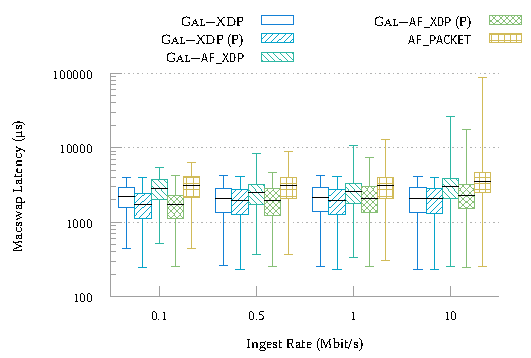
\includegraphics[keepaspectratio,width=\resultplotwidth]{../plots/build/latency-vs-baselines/rpi-64B-trimlog-new}
	\caption{Macswap latency distributions for \qty{64}{\byte} packets on \emph{RPi} for \ourtech{} vs.\ \afp{}. The XDP fast path outperforms \afp{}, has better tail latencies at higher rates, and improves by polling at low data rates.\label{fig:lat-rpi}}
\end{figure}

\begin{figure*}
	\centering
	\subfloat[\emph{IRQ}\label{fig:lat-nuc:irq}]{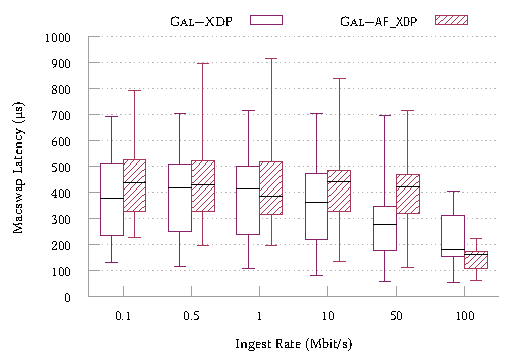
\includegraphics[keepaspectratio,width=0.48\linewidth]{../plots/build/latency-vs-baselines/nuc-64B-wide-irq-new}}
	\subfloat[\emph{Poll\label{fig:lat-nuc:poll}}]{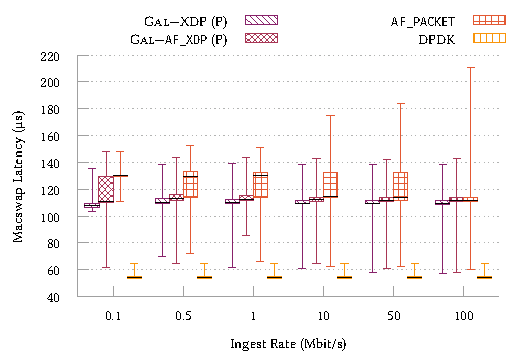
\includegraphics[keepaspectratio,width=0.48\linewidth]{../plots/build/latency-vs-baselines/nuc-64B-wide-poll-new}}
	
%	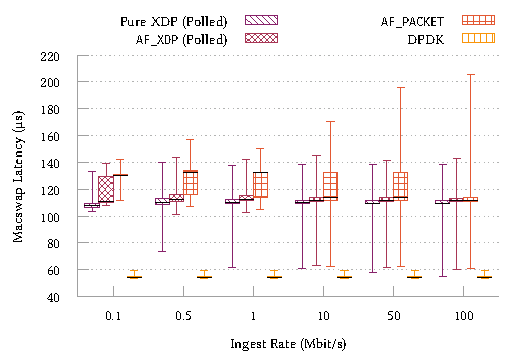
\includegraphics[keepaspectratio,width=0.5\linewidth]{../plots/build/latency-vs-baselines/nuc-64B-wide-poll}
	\caption{Macswap latency distributions for \qty{64}{\byte} packets on an Intel NUC for \ourtech{} vs.\ \afp{} and DPDK. XDP consistently outperforms \afxdp{}, with both seeing improvements at higher traffic rates. Polling improves the performance of \ourtech{} beyond \afp{}, but cannot beat DPDK.\label{fig:lat-nuc}}
\end{figure*}

\begin{table}
	\caption{Raspberry Pi Macswap NF throughput and resource use, \qty{64}{\byte} packets.\label{tab:rpi-64}}
		
	\resizebox{\linewidth}{!}{\expandableinput{../tables/build/vs-baselines-new/rpi-64B-ex100.tex}}
	
%	\resizebox{\linewidth}{!}{\expandableinput{../tables/build/vs-baselines/rpi-256B.tex}}
	
%	\resizebox{\linewidth}{!}{\expandableinput{../tables/build/vs-baselines/rpi-512B.tex}}
%
%	\resizebox{\linewidth}{!}{\expandableinput{../tables/build/vs-baselines/rpi-1280B.tex}}
%	
%	\resizebox{\linewidth}{!}{\expandableinput{../tables/build/vs-baselines/rpi-1518B.tex}}
\end{table}

%\begin{table}
%	\caption{Raspberry Pi Macswap NF throughput and resource use, \qty{512}{\byte} packets.\label{tab:rpi-512}}
%	
%	\resizebox{\linewidth}{!}{\expandableinput{../tables/build/vs-baselines-new/rpi-512B.tex}}
%\end{table}

\begin{table}
	\caption{Raspberry Pi Macswap NF throughput and resource use, \qty{1518}{\byte} packets.\label{tab:rpi-1518}}
	
%	\resizebox{\linewidth}{!}{\expandableinput{../tables/build/vs-baselines/rpi-64B-ex100.tex}}
	
	%	\resizebox{\linewidth}{!}{\expandableinput{../tables/build/vs-baselines/rpi-256B.tex}}
	
%	\resizebox{\linewidth}{!}{\expandableinput{../tables/build/vs-baselines/rpi-512B.tex}}
	
%	\resizebox{\linewidth}{!}{\expandableinput{../tables/build/vs-baselines-new/rpi-1280B.tex}}
	
	\resizebox{\linewidth}{!}{\expandableinput{../tables/build/vs-baselines-new/rpi-1518B.tex}}
\end{table}

%?? Talk abt latencies
%?? \cref{fig:lat-rpi,fig:lat-nuc}
\Cref{fig:lat-rpi} shows the distribution of packet latencies on \emph{RPi}, up to its peak stable throughput for \qty{64}{\byte} packets.
We see that \ourtech{}'s XDP fast path significantly outperforms \afp{}---\qtyrange{29}{41}{\percent} lower median latencies for \qtylist{0.1;10}{\mega\bit\per\second} (\qtyrange{36.1}{95.4}{\percent} reduction at \nth{99} percentile) without polling.
%?? RPi: XDP \qty{29}{\percent} lower median at 0.1, \qty{34}{\percent} lower median at 10 vs afp
%?? RPi: XDP \qty{31.2}{\percent} lower 99th at 0.1, \qty{92.6}{\percent} lower 99th at 10 vs afp -- IRQ-based AFP is \qty{54.3}{\percent} lower.
%?? RPI: \afxdp{} is a latency midpoint at median at moderate data rates, loses out at more stress (better tail than afp).
At moderate data rates, the userland datapath (\afxdp{}) falls between these two extremes, tending towards \afp's median behaviour under stress (with better tail behaviour).
%?? RPi: Lower mins at higher pkt rates due to USB behaviour -- hampered universally.
Higher ingest rates lead to lower minimum latencies (i.e., a few packets benefit from batching), but have limited impact on median XDP latencies (\qty{5.5}{\percent}) and a slight adverse impact on \afxdp---performance is mainly governed by the USB polling interval.
%?? RPi: 50Mbps ingest causes mean latencies to increase by \qty{100}{\times} (not shown), noting that the device cannot sustain this rate (\cref{tab:rpi-64}).
Overloading ingest (e.g., $\ge$\qty{50}{\mega\bit\per\second}) causes median latencies to increase by \qty{100}{\times} (plot omitted).

\begin{table}
	\caption{Intel NUC Macswap NF throughput and resource use, \qty{64}{\byte} packets.\label{tab:nuc-64}}
	
	\resizebox{\linewidth}{!}{\expandableinput{../tables/build/vs-baselines-new/nuc-64B.tex}}
%	\resizebox{\linewidth}{!}{\expandableinput{../tables/build/vs-baselines/nuc-64B.tex}}
	
	%	\resizebox{\linewidth}{!}{\expandableinput{../tables/build/vs-baselines/nuc-1518B.tex}}
\end{table}

\Cref{fig:lat-nuc:irq} shows that, on Intel NUCs, the XDP fast path offers a \qtyrange{100}{150}{\micro\second} median improvement over the userland datapath, where latencies improve at higher ingest rates in both cases.
However, at \qty{1}{\giga\bit\per\second} XDP's median--\nth{99} latencies increase to \qtyrange{1978.2}{2008.7}{\micro\second} regardless of polling, with \afxdp{} \qty{1.44}{\times} worse (plot omitted).
When polling for packets (\cref{fig:lat-nuc:irq}), both of \ourtech{}'s datapaths outperform \afp{}, but exhibit around \qty{2}{\times} the overhead of DPDK.
%?? NUC: DPDK always wins, but still benefits for placing NFs in XDP vs \afxdp{}.

%?? Talk abt tputs.
We see that \ourtech{}'s dataplanes can sustain traffic on \emph{RPi} at \qtylist[list-units = single]{10;50;100}{\mega\bit\per\second} for \qtylist[list-units = single]{64;512;1518}{\byte} packets respectively (\cref{tab:rpi-64,tab:rpi-1518}).
%(\cref{tab:rpi-64,tab:rpi-512,tab:rpi-1518}).
\afp{} fails to meet \qty{50}{\mega\bit\per\second} for \qty{512}{\byte} packets (table omitted). %, noting that forwarding throughput at the latter rate falls to 0 for packets sizes above \qty{1280}{\byte}. ?? FIXME: not anymore!! But it does require more CPU and power than \afp.
\emph{NUC} is able to meet \qty{1}{\giga\bit\per\second} traffic for all packet sizes and dataplane designs except \afp{} (\cref{tab:nuc-64}).
We see sub-linerate results here as we include the startup and winddown of traffic generation---manual testing with Pktgen-DPDK confirms that our dataplanes and DPDK sustain \qty{1}{\giga\bit\per\second} at peak.
%?? TODO: manually test some max pps numbers.

%?? CPU/Power?
On \emph{RPi} (IRQ), we see lower like-for-like CPU and power use as compared with \afp{} (\cref{tab:rpi-64}).
For \qty{1518}{\byte} packets in the same case, we see that the pure XDP datapath offers up to \qty{3.1}{\times} CPU reduction versus userland, requiring \qty{7.4}{\percent} less power (\cref{tab:rpi-1518}).
We interpret this effect as arising from copying packet contents into UMEM frames, however this remains lower than \afp.
%?? Lower like-for-like CPU use on RPi vs \afp{} baseline i.e. at same ingest rate.
However, while \ourtech{} CPU use is lower than \afp{} when polling, we observe that XDP dataplanes have around \qty{5}{\percent} higher power use.
%?? NUC: fast-path far more CPU-efficient (\cref{tab:nuc-64})
%?? NUC: poll basically always consumes a core (\cref{tab:nuc-64})
In \emph{NUC}, we see that the fastpath is always more CPU-efficient for rates beyond \qty{1}{\mega\bit\per\second} (\cref{tab:nuc-64}).

\fakepara{Takeaways}
\ourtech{} is well-suited to non-DPDK capable devices such as Raspberry Pis, offering better overall performance in both its datapaths (and lower power/CPU use) than frameworks like \afp.
Polling offers limited benefits on the Raspberry Pi, and cannot beat best-of-breed solutions like DPDK when they are supported---however, it is already understood that XDP underperforms in this comparison, but is far more CPU-efficient at lower traffic rates~\parencite{DBLP:journals/tnsm/MianoRBBL21,DBLP:conf/conext/Hoiland-Jorgensen18} (i.e., those of interest in IoT/sensor networks).
\ourtech{} benefits most from the CPU and power reductions of blocking I/O to support portable, \emph{efficient}, in-situ traffic processing.
%?? DPDK always better for latency, but everyone knows this.
%?? XDP is well-understood to achieve lower throughput and worse latency than DPDK, but is far more CPU-efficient at lower traffic rates~\parencite{DBLP:journals/tnsm/MianoRBBL21,DBLP:conf/conext/Hoiland-Jorgensen18}.
%?? As a single universally-supported framework, this works best on DPDK-platforms where we want to minimise CPU (ergo power) use

\subsection{Scheduling expensive NFs}
\begin{figure}
	\centering
	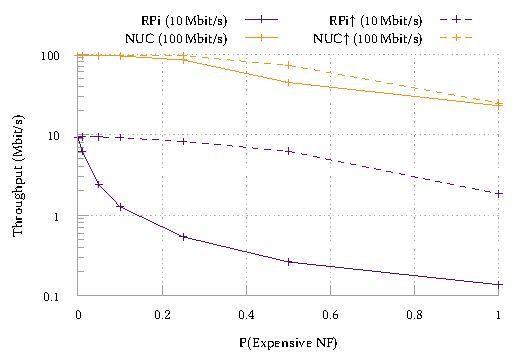
\includegraphics[keepaspectratio,width=\resultplotwidth]{../plots/build/blocking-xdp/tput-degrade-10-new}
	\caption{Throughput degradation as compute-intense NFs are run in the XDP path. `$\uparrow$' denotes passing such packets to userland. Expensive NFs cause significant throughput loss---strongest for \emph{RPi}---but are alleviated using \ourtech{}'s two-tier datapath strategy.\label{fig:tput-degrade}}
\end{figure}

\begin{figure}
	\centering
	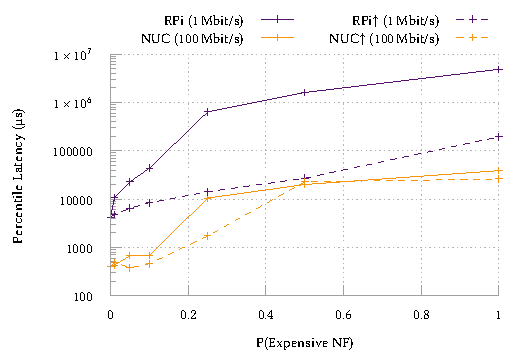
\includegraphics[keepaspectratio,width=\resultplotwidth]{../plots/build/blocking-xdp/lat-degrade-99-new}
	\caption{\nth{99} percentile latency degradation, as in \cref{fig:tput-degrade}. For \emph{RPi}, offloading costly NFs to userland offers \numrange{1}{2} orders of magnitude improvement.\label{fig:lat-degrade}}
\end{figure}

Compute-intense NFs, as hypothesised, significantly harm median/\nth{99} percentile latencies and overall throughputs if applied in the XDP fast path to even \qty{1}{\percent} of packets.
\Cref{fig:tput-degrade,fig:lat-degrade} show this property for throughput and \nth{99} percentile latencies respectively on peak traffic for each SBC---\emph{RPi} is more adversely affected (having a slower CPU clock), but unlike \emph{NUC} even lower traffic rates are impacted (\qtylist[list-units=single]{0.5;1}{\mega\bit\per\second}, plot omitted).
Crucially, pushing costly NFs to userland alleviates this problem, particularly on weaker SBCs (i.e., a \qty{25.7}{\times} increase in throughput for \emph{RPi}, $P=$~\num{0.5}).

%We see that the effect of compute intense NFs is naturally stronger in devices with slower CPU clocks 

%?? Multicore bad for small NFs, but larger?
We find the value of additional cores for load balancing depends on NF complexity.
In earlier experiments, we found for \emph{RPi} that the split-datapath design could not improve throughputs beyond pure XDP for cheaper NF chains (i.e., bottlenecked by kernel packet handling), while on \emph{NUC} the XDP dataplane could already handle all rates with ease in spite of having a single queue.
In addition, we found there to be some contention when reading from the separate \afxdp{} sockets in userland which limits the applicability of load-balancing cheaper NFs in this way.
However, more expensive NFs are a prime candidate for placement over the unused device cores---we see from \cref{fig:tput-cores} that additional threads are serving as many packets as possible.

\begin{figure}
	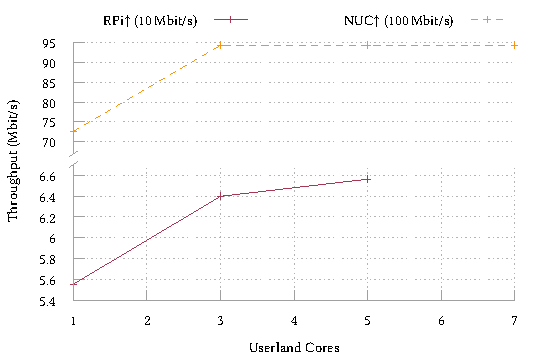
\includegraphics[keepaspectratio,width=\resultplotwidth]{../plots/build/core-allev-block/tput-split}
	\caption{Extra userland cores lead to improved throughput as more packets ($P=$~\num{0.5}) require expensive NFs. 64B packets.\label{fig:tput-cores}}
\end{figure}

\fakepara{Takeaways}
The two-tier split datapath design of \ourtech{} is key in ensuring that SBCs can provide different quality of service to packets which require different levels of processing, and for protecting `normal' traffic from latency spikes and drops caused by expensive analyses on adversarial flows.

\section{Related Work}\label{sec:related}

\fakepara{SBC dataplanes}
\emph{P4Pi}~\parencite{DBLP:journals/ccr/LakiSKSVZ21} is an educational platform to run P4 dataplanes on Rasbperry Pi devices.
Its dataplane uses DPDK on tap devices bridged from the onboard NICs (similar to our \afp{} baseline), and is limited to the simpler semantics of P4 programs versus our eBPF-plus-native code strategy.
P4Pi and \ourtech{} have altogether different aims and are complementary to one another; given our results, P4Pi might reduce its power costs and latency using \af{}.

\fakepara{eBPF/XDP dataplanes}
\emph{Polycube}~\parencite{DBLP:journals/tnsm/MianoRBBL21} uses a similar hybrid XDP-userland model to provide SFC in datacentres.
While both \ourtech{} and Polycube rely on chains of tail-calls between XDP programs, \citeauthor{DBLP:journals/tnsm/MianoRBBL21} designate an explicit userland component per NF.
If userland processing is required, Polycube upcalls packets using per-CPU ring buffers, and then \emph{recirculates packets back to the XDP datapath} using tap devices.
\ourtech{} is instead tailored towards SBC devices.
We use \afxdp{} for upcalling due to its ubiquity and robustness---and never return packets to XDP due to the single XDP thread offered by SBC hardware.
Both frameworks are specialised toward their target environment (datacentres vs.\ SBCs).

\emph{Morpheus}~\parencite{DBLP:conf/asplos/MianoSRRA22} examines how runtime profiling can improve the performance of eBPF-based dataplanes via \emph{profile guided optimisation}.
While the improvements it offers would complement our work, this relies on routinely sending instrumentation data back to \ourtech{}'s compile server---and so would require more in-depth cost/benefit analysis of network overheads.

%\ourtech{} cannot efficiently pass packets back to XDP due to the limited count of hardware receive queues on SBC hardware.
%
% + \emph{Morpheus}~\parencite{DBLP:conf/asplos/MianoSRRA22}
%?? Similarities: also SFC in an XDP context (eBPF NFs with userland as needed), also reliant on tail-calls.
%?? How do we differ from Sebi's work? -- We make use of \afxdp{} to pass packets, while they use (per-cpu perf ring buffers?).
%?? They downcall via tap devices \emph{every time a slow-path operation completes}, and assume that programs are already provided as precompiled programs. Full-source-code allows better `universal' deploy. We don't recirc, and don't explicitly have a `routing phase' between NFs -- the call graph is defined 
%?? Why don't we recirc? 
%%?? We require no extra BPF helpers which are needed for up/downcalls in their scheme.
%?? BPF Compiler Collection (BCC) on C programs.

%?? Decomposition~\parencite{DBLP:conf/conext/ShahinfarMSSBA21} works because they're implicitly getting a pipelining effect over several cores.

\Textcite{DBLP:conf/conext/ShahinfarMSSBA21} have seen some performance benefits in splitting packet processing between XDP and userland via \afxdp.
We believe that this is due to the same `pipeline parallelism' that \ourtech{} takes advantage of.

\fakepara{eBPF in industry}
eBPF's safety, performance, and kernel integration make it useful in many applications.
\emph{Cilium}~\parencite{cilium} uses XDP to insert security and load balancing functions into container networks.
\emph{flowtrackd}~\parencite{flowtrackd} uses \afxdp{} to provide DDoS attack scrubbing capabilities for Cloudflare CDNs.
\emph{Open vSwitch}~\parencite{DBLP:conf/sigcomm/TuWAP21} has been redesigned to make use of \afxdp{} for its agility over kernel modules, while load balancers like \emph{Katran}~\parencite{katran} are in widespread deployment in Meta.

\fakepara{Rust-based dataplanes}
\emph{NetBricks}~\parencite{DBLP:conf/osdi/PandaHJWRS16} installs SFC graphs of Rust NFs over the DPDK dataplane.
It offers effective abstractions for aggregating and processing traffic---however, it does not provide any mechanisms or support for an eBPF/XDP dataplane.
\emph{SafeBricks}~\parencite{DBLP:conf/nsdi/PoddarLPR18} protects these NFs from a compromised kernel using TEEs, however these are absent in Raspberry Pis and deprecated in consumer Intel CPUs~\parencite{sgx-depr}.

%?? Mention eBPF limitations... vs their NF limitations

\section{Conclusion}
We have presented \ourtech, an SFC framework designed for the cheap defence of IoT networks.
By carefully considering the limitations of the XDP framework on SBC hardware, we have designed and implemented an SFC framework tailored to making the best use of SBC parallelism while protecting `normal' traffic.
We have empirically shown that our design achieves lower and more consistent latencies on weaker SBC devices like Raspberry Pis, enabling inexpensive NF installation in IoT and sensor networks.

\fakepara{Acknowledgements}
This work was supported in part by the PETRAS National Centre of Excellence for IoT Systems Cybersecurity, via the UK Engineering and Physical Sciences
Research Council [grant EP/S035362/1].

\printbibliography

\end{document}